\chapter{Process Analysis}

As we are now at the end of the project, we want to talk a bit about the process, planning and the outcome from this project.


\section{Project Planning}
\label{ProjectPlanning}
As we have already mentioned in section \ref{WorkProcess} we used the kanbanflow tool to manage our tasks and work flow for this project. All red tasks are programming/product oriented, where the yellow ones are report/documentation related. The plan did change slightly a few times due to new acquired knowledge on the topic, and thereby forcing us to change the schedule slightly. Each change has always been made after an iteration has ended, as changing the schedule midway through an iteration is often wrong to do when working in iterations.

We saw in section \ref{WorkProcess} how we initially planned out our project, but we did underestimate how much we could do in 3 weeks. Already after a week into the project period, we had already completed most of the initial work of writing the introduction chapters, as well as programming most of the planned tasks for that iteration. We then began to take task from iteration 2 and slowly also empty out the second iteration, and at the end of our first iteration we ended up with the schedule seen in \figref{fig:afteritration1}.

\begin{figure}[H]
	\includegraphics[width=1.0\linewidth]{img/afteriteration1}
	\centering
	\caption{Our schedule after iteration 1}
	\label{fig:afteritration1}
\end{figure}

As we in the schedule in \figref{fig:afteritration1} were almost a half iteration ahead, we modified it to better match our current situation. As we in iteration 1 also got to look into some articles about procedural content generation, we got new knowledge about the topic, and realized that a few changes were necessary. As we can see in \figref{fig:BeforeIteration2}, we moved implementation from iteration 2 to 3 and added a new task to iteration 2 about noise manipulation. We did also find out that the second task that was in progress was very huge, and there was much more to them than we first thought, so we added in subtasks to both of them. By adding subtasks we also found that a few already existing tasks should be a subtask rather than a task for it self.

\begin{figure}[H]
	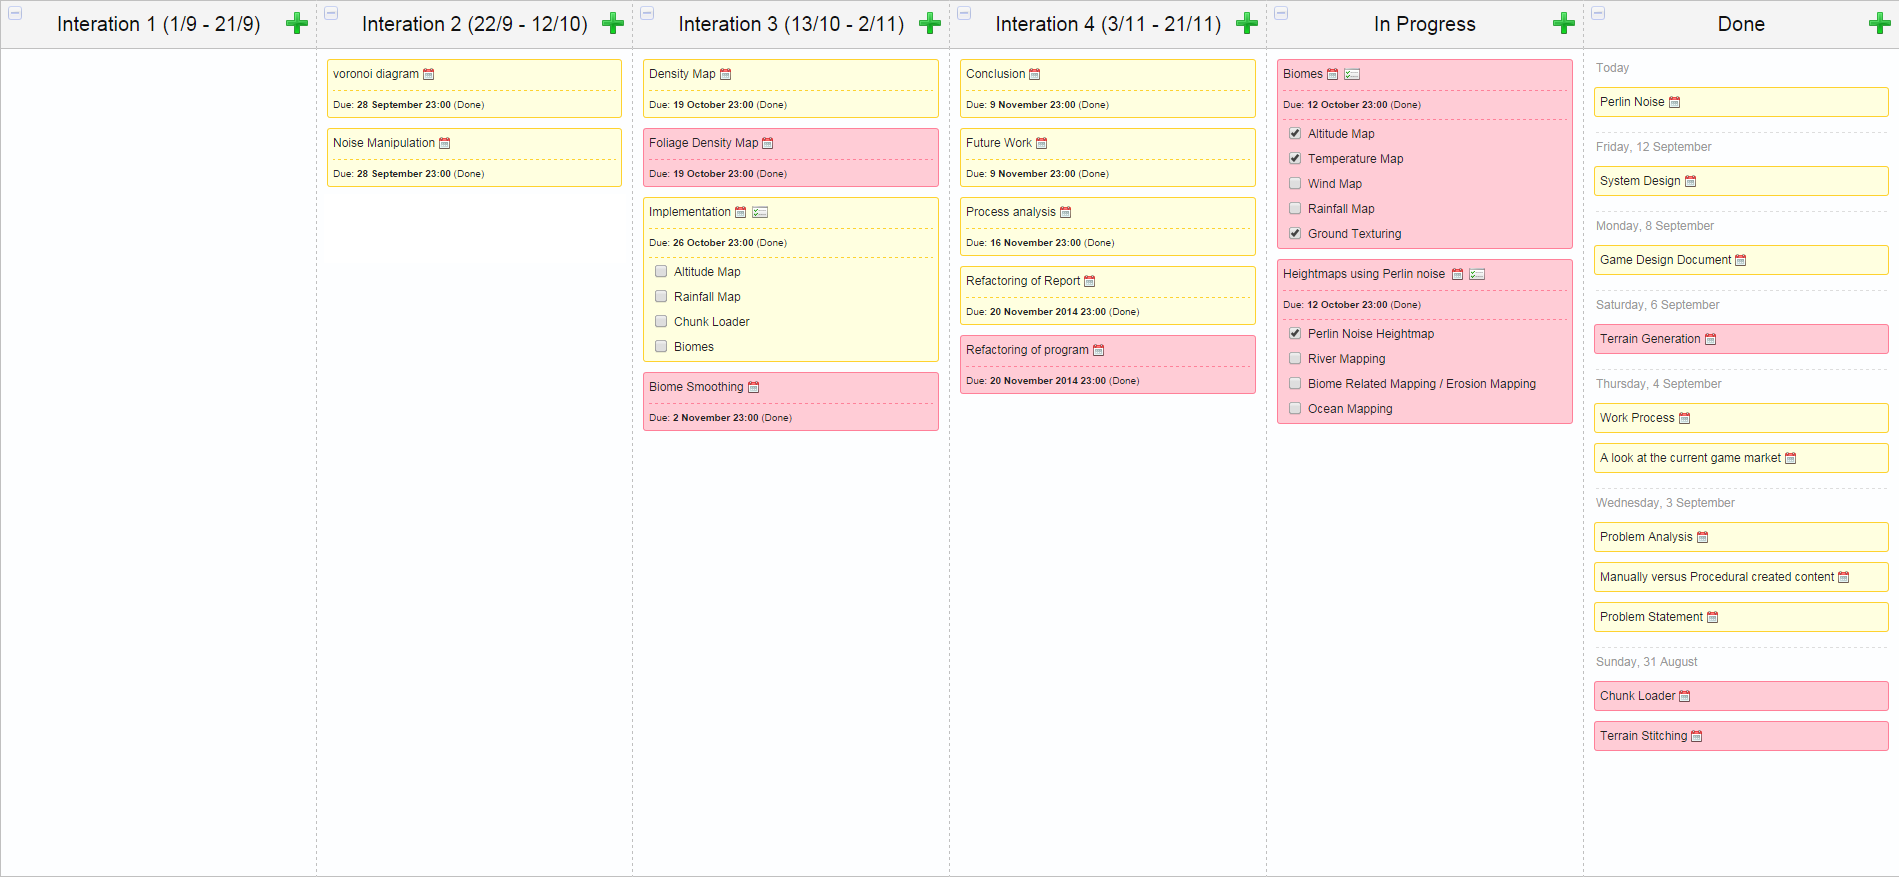
\includegraphics[width=1.0\linewidth]{img/BeforeIteration2}
	\centering
	\caption{Our schedule readjusted for iteration 2}
	\label{fig:BeforeIteration2}
\end{figure}

The reason we did not add more than one new task to iteration 2, is due to the fact that the 2 current in progress tasks were very huge and we needed much more time to certain subtasks. Due to this we decided to be vary with how many tasks we had for the second iteration.

As we reached the end of iteration 2 we were slightly behind our schedule as seen in \figref{fig:BeforeIteration3}. We believe that the choices made to the schedule may have decreased the amount of work we were behind. Even though we were slightly behind we didn't feel the need to change the schedule, and started iteration 3 as we left iteration 2.

\begin{figure}[H]
	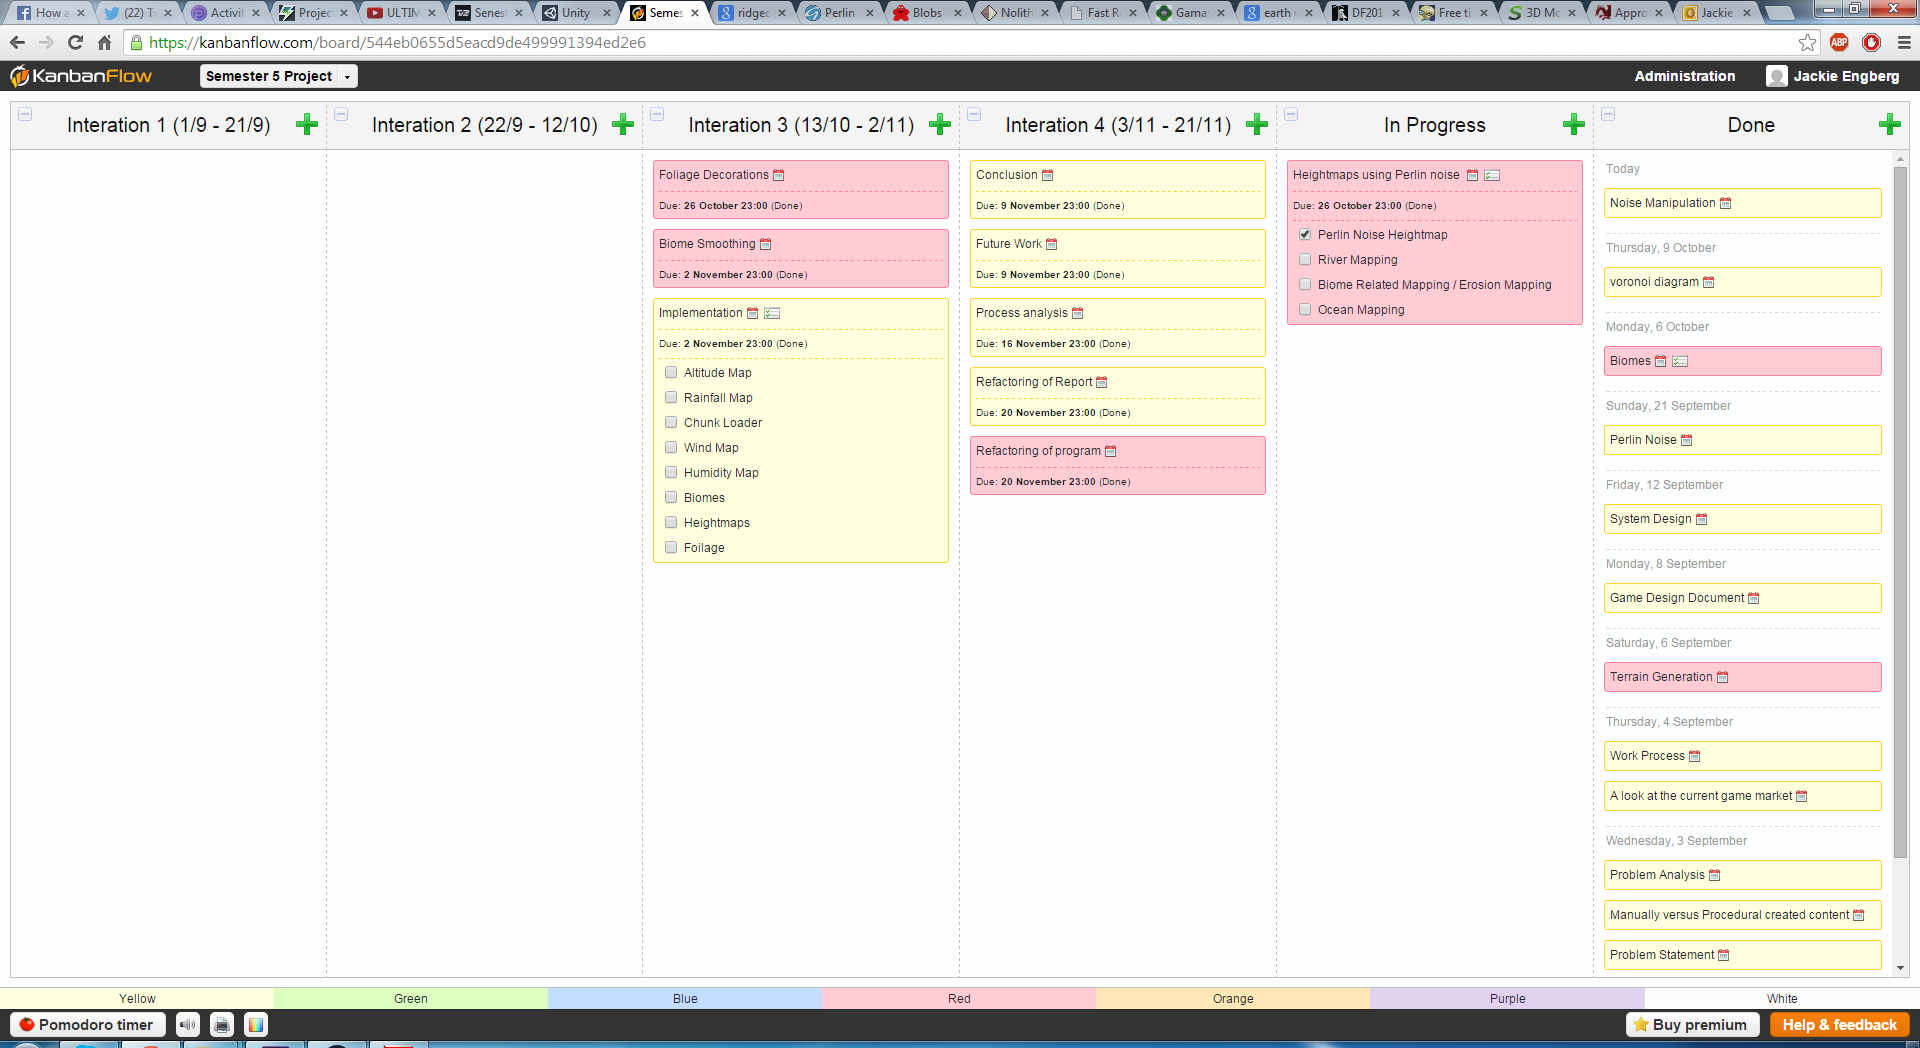
\includegraphics[width=1.0\linewidth]{img/BeforeIteration3}
	\centering
	\caption{Our schedule at the end of iteration 2}
	\label{fig:BeforeIteration3}
\end{figure}

At the end of iteration 3, the schedule was all in order and we were on time as expected in the original schedule and we went into the 4th and last iteration without any changes made.


\section{Learning Outcome}

We went into this project with a little background knowledge on how procedural content generation worked in general, but after having worked with it full time for multiple weeks we now know a lot more. We have learned how we from code, randomly can create billions of infinite worlds, and levels which also has some sort of diversity. We have also learned a lot from our mistakes, and have a few gray areas that we now also have the knowledge to fix in the future, however, due to the strict time limit of the project, it is limited to what is possible to make within that timespan as games can take years to make stable enough to have a public release.